\documentclass[a4paper,
fontsize=11pt,
%headings=small,
oneside,
numbers=noperiodatend,
parskip=half-,
bibliography=totoc,
final
]{scrartcl}

\usepackage[babel]{csquotes}
\usepackage{synttree}
\usepackage{graphicx}
\setkeys{Gin}{width=.4\textwidth} %default pics size

\graphicspath{{./plots/}}
\usepackage[ngerman]{babel}
\usepackage[T1]{fontenc}
%\usepackage{amsmath}
\usepackage[utf8x]{inputenc}
\usepackage [hyphens]{url}
\usepackage{booktabs} 
\usepackage[left=2.4cm,right=2.4cm,top=2.3cm,bottom=2cm,includeheadfoot]{geometry}
\usepackage{eurosym}
\usepackage{multirow}
\usepackage[ngerman]{varioref}
\setcapindent{1em}
\renewcommand{\labelitemi}{--}
\usepackage{paralist}
\usepackage{pdfpages}
\usepackage{lscape}
\usepackage{float}
\usepackage{acronym}
\usepackage{eurosym}
\usepackage{longtable,lscape}
\usepackage{mathpazo}
\usepackage[normalem]{ulem} %emphasize weiterhin kursiv
\usepackage[flushmargin,ragged]{footmisc} % left align footnote
\usepackage{ccicons} 
\setcapindent{0pt} % no indentation in captions

%%%% fancy LIBREAS URL color 
\usepackage{xcolor}
\definecolor{libreas}{RGB}{112,0,0}

\usepackage{listings}

\urlstyle{same}  % don't use monospace font for urls

\usepackage[fleqn]{amsmath}

%adjust fontsize for part

\usepackage{sectsty}
\partfont{\large}

%Das BibTeX-Zeichen mit \BibTeX setzen:
\def\symbol#1{\char #1\relax}
\def\bsl{{\tt\symbol{'134}}}
\def\BibTeX{{\rm B\kern-.05em{\sc i\kern-.025em b}\kern-.08em
    T\kern-.1667em\lower.7ex\hbox{E}\kern-.125emX}}

\usepackage{fancyhdr}
\fancyhf{}
\pagestyle{fancyplain}
\fancyhead[R]{\thepage}

% make sure bookmarks are created eventough sections are not numbered!
% uncommend if sections are numbered (bookmarks created by default)
\makeatletter
\renewcommand\@seccntformat[1]{}
\makeatother

% typo setup
\clubpenalty = 10000
\widowpenalty = 10000
\displaywidowpenalty = 10000

\usepackage{hyperxmp}
\usepackage[colorlinks, linkcolor=black,citecolor=black, urlcolor=libreas,
breaklinks= true,bookmarks=true,bookmarksopen=true]{hyperref}
\usepackage{breakurl}

%meta
%meta

\fancyhead[L]{J. Zaugg, Red. LIBREAS\\ %author
LIBREAS. Library Ideas, 38 (2020). % journal, issue, volume.
\href{http://nbn-resolving.de/}
{}} % urn 
% recommended use
%\href{http://nbn-resolving.de/}{\color{black}{urn:nbn:de...}}
\fancyhead[R]{\thepage} %page number
\fancyfoot[L] {\ccLogo \ccAttribution\ \href{https://creativecommons.org/licenses/by/4.0/}{\color{black}Creative Commons BY 4.0}}  %licence
\fancyfoot[R] {ISSN: 1860-7950}

\title{\LARGE{9 Fragen an die Illustratorin Judith Zaugg}}% title
\author{Judith Zaugg, Redaktion LIBREAS} % author

\setcounter{page}{1}

\hypersetup{%
      pdftitle={9 Fragen an die Illustratorin Judith Zaugg},
      pdfauthor={Judith Zaugg, Redaktion LIBREAS},
      pdfcopyright={CC BY 4.0 International},
      pdfsubject={LIBREAS. Library Ideas, 38 (2020).},
      pdfkeywords={Interview, Bibliothek, Kunst, Kommunikation, Illustration},
      pdflicenseurl={https://creativecommons.org/licenses/by/4.0/},
      pdfcontacturl={http://libreas.eu},
      baseurl={http://libreas.eu},
      pdflang={de},
      pdfmetalang={de}
     }



\date{}
\begin{document}

\maketitle
\thispagestyle{fancyplain} 

%abstracts

%body
Vielen Dank, dass Sie sich bereit erklärt haben, unsere Fragen zu
beantworten. Wir haben gemerkt, dass eine ganze Anzahl von
Designer*innen und Künstler*innen, wenn sie für Bibliotheken arbeiten,
gerne als ein Symbol auf Tiere oder Pflanzen zurückgreifen. Uns
interessiert, warum das so ist. Gleichzeitig wollen wir die Möglichkeit
nutzen, um von ihrer Seite zu hören, wie eine solche Zusammenarbeit mit
Bibliotheken abläuft.

\emph{LIBREAS: Wann kamen Sie das erste Mal in Ihrer Arbeit mit
Bibliotheken in Kontakt? Hatte das bei Ihnen \enquote{Vorläufer},
beispielsweise eigene Erfahrungen aus der Kindheit?}

Es war die Bibliothek meiner Kindheit, also von meinem Wohnquartier, die
mich für einen Vortrag über meine Illustrationsarbeit eingeladen hat.

\emph{LIBREAS: Wie kam der Kontakt für diese beiden
bibliotheksspezifischen Projekte zustande? Sind Sie mit Ideen auf die
Einrichtungen zugegangen oder kamen die zu ihnen? War das der normale
Weg, wie solche Projekte zustande kommen oder eher ungewöhnlich?}

Ich wurde von der jeweiligen Bibliothek angefragt, was mich eigentlich
der ganz übliche Weg ist.

\emph{LIBREAS: Unterscheiden sich für Sie als Designerin Bibliotheken
als Kund*innen von anderen Einrichtungen?}

Ja, am Anfang von meiner Arbeit als Grafikerin und Illustratorin war
noch alles analog. Das bedeutet, dass ich für Vorlagen oder
Informationen zu bestimmten Themen sehr auf die Bibliotheken angewiesen
war.

\emph{LIBREAS: Wir haben, wenn wir ehrlich sind, wenig Ahnung von einem
solchen Design-Prozess. Wie gehen Sie allgemein vor, um zu Motiven für
solche Arbeiten zu gelangen? Und wie sind Sie bei dieser konkreten
Arbeit zu diesen Motiven gelangt?}

Für die Lesezeichen für die Schweizerische Nationalbibliothek sass ich
mit der Projektverantwortlichen zusammen. Sie wollte vier Motive von
mir, die Leser*innen auf künstlerische, freundliche und witzige Art
darauf aufmerksam machen, dass sie zu den Büchern Sorgfalt tragen
müssen.

Die Vorgaben für die Darstellung waren, dass

\begin{enumerate}
\def\labelenumi{\arabic{enumi}.}
\item
  man die Bücher nicht kopieren soll, sondern abschreiben,
\item
  man keine klebenden oder zum Beispiel metalligen Lesezeichen wie
  Büroklammern verwenden soll, sondern nur Lesezeichen aus Papier,
\item
  man die Bücher nicht für andere als buchtypische Zwecke verwenden soll
\item
  man beim Lesen nicht essen und trinken soll.
\end{enumerate}

Die Idee der Bibliothek war, dass jedes Jahr so eine Serie mit vier
Lesezeichen von jeweils einer anderen Künstler*in gestaltet wird. Ich
war die Erste. Die Lesezeichen waren ein Erfolg, aber die Serie wurde
leider nicht fortgesetzt.

\begin{figure}[h!]
\centering
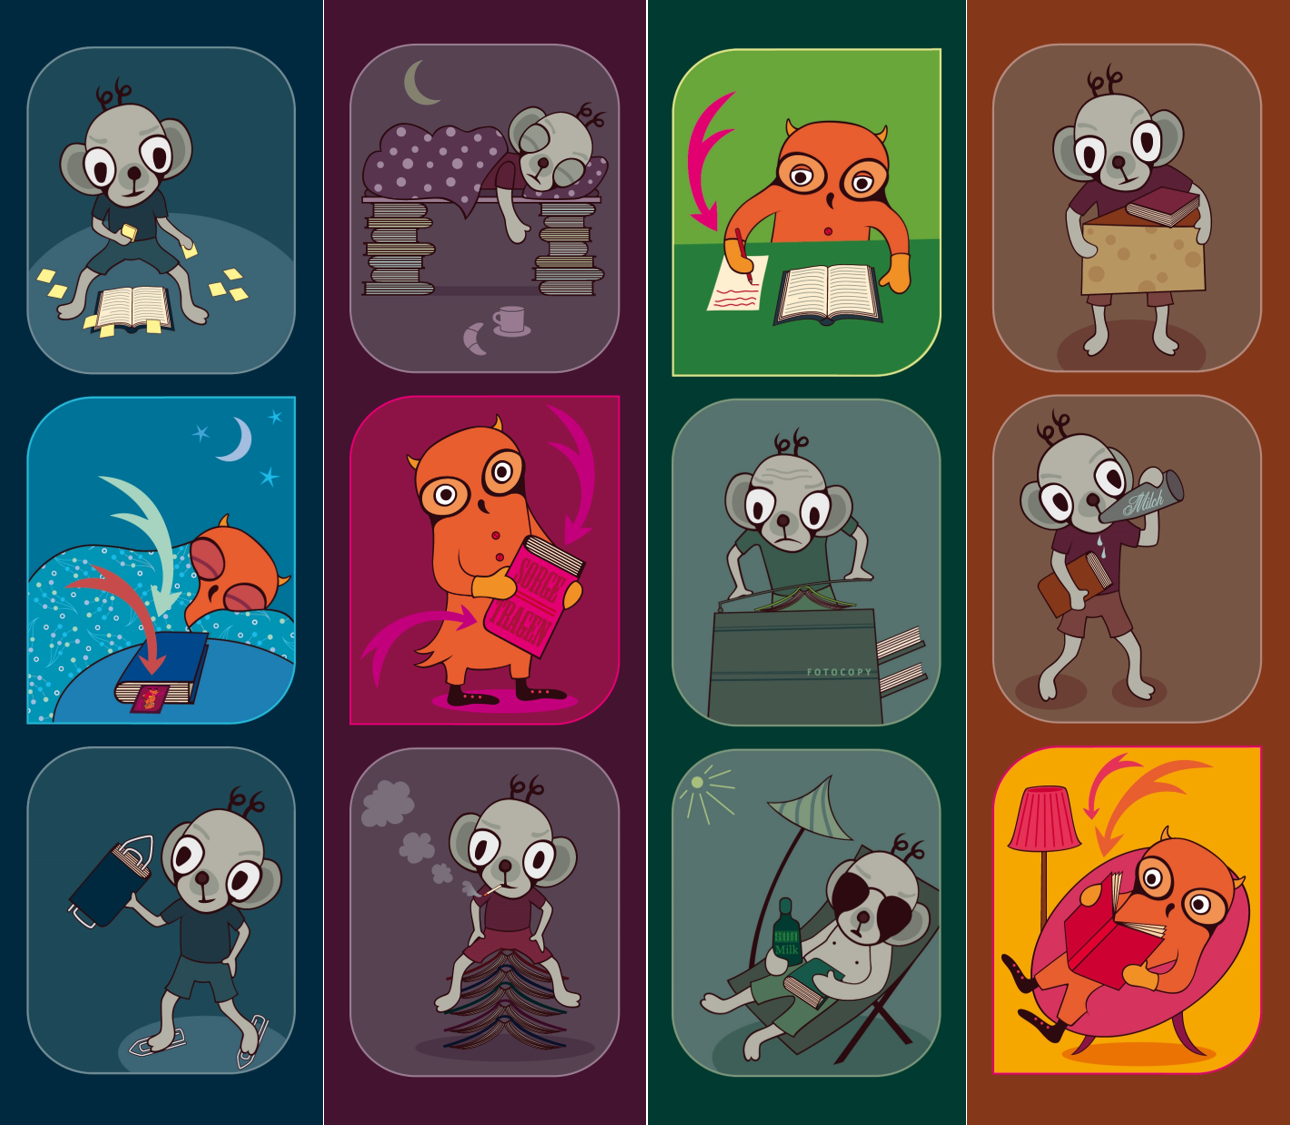
\includegraphics[width=0.9\textwidth]{img/image1.png}
\end{figure}

Für die Kornhausbibliotheken in Bern durfte ich vier Postkarten
gestalten :

\begin{itemize}
\item
  zwei Geschenkgutscheine (Weihnachtsmotiv und Ganzjahresmotiv)
\item
  zwei Varianten eines Gutschein Buchstart-Pakets für Eltern zur Geburt
  ihres Kindes.
\end{itemize}

Auch hier sass ich mit der Bibliotheksleiterin für ein gemeinsames
Brainstorming zusammen und wir haben ein Brainstorming gemacht. Danach
entwarf ich die Karten als Bleistiftzeichnungen. Die Kundin war von
Beginn an zufrieden und ich habe die Reinzeichnung im Programm Adobe
Illustrator gemacht.

Das Vorgehen ähnelte sich also bei beiden Aufträgen.

\begin{figure}[h!]
\centering
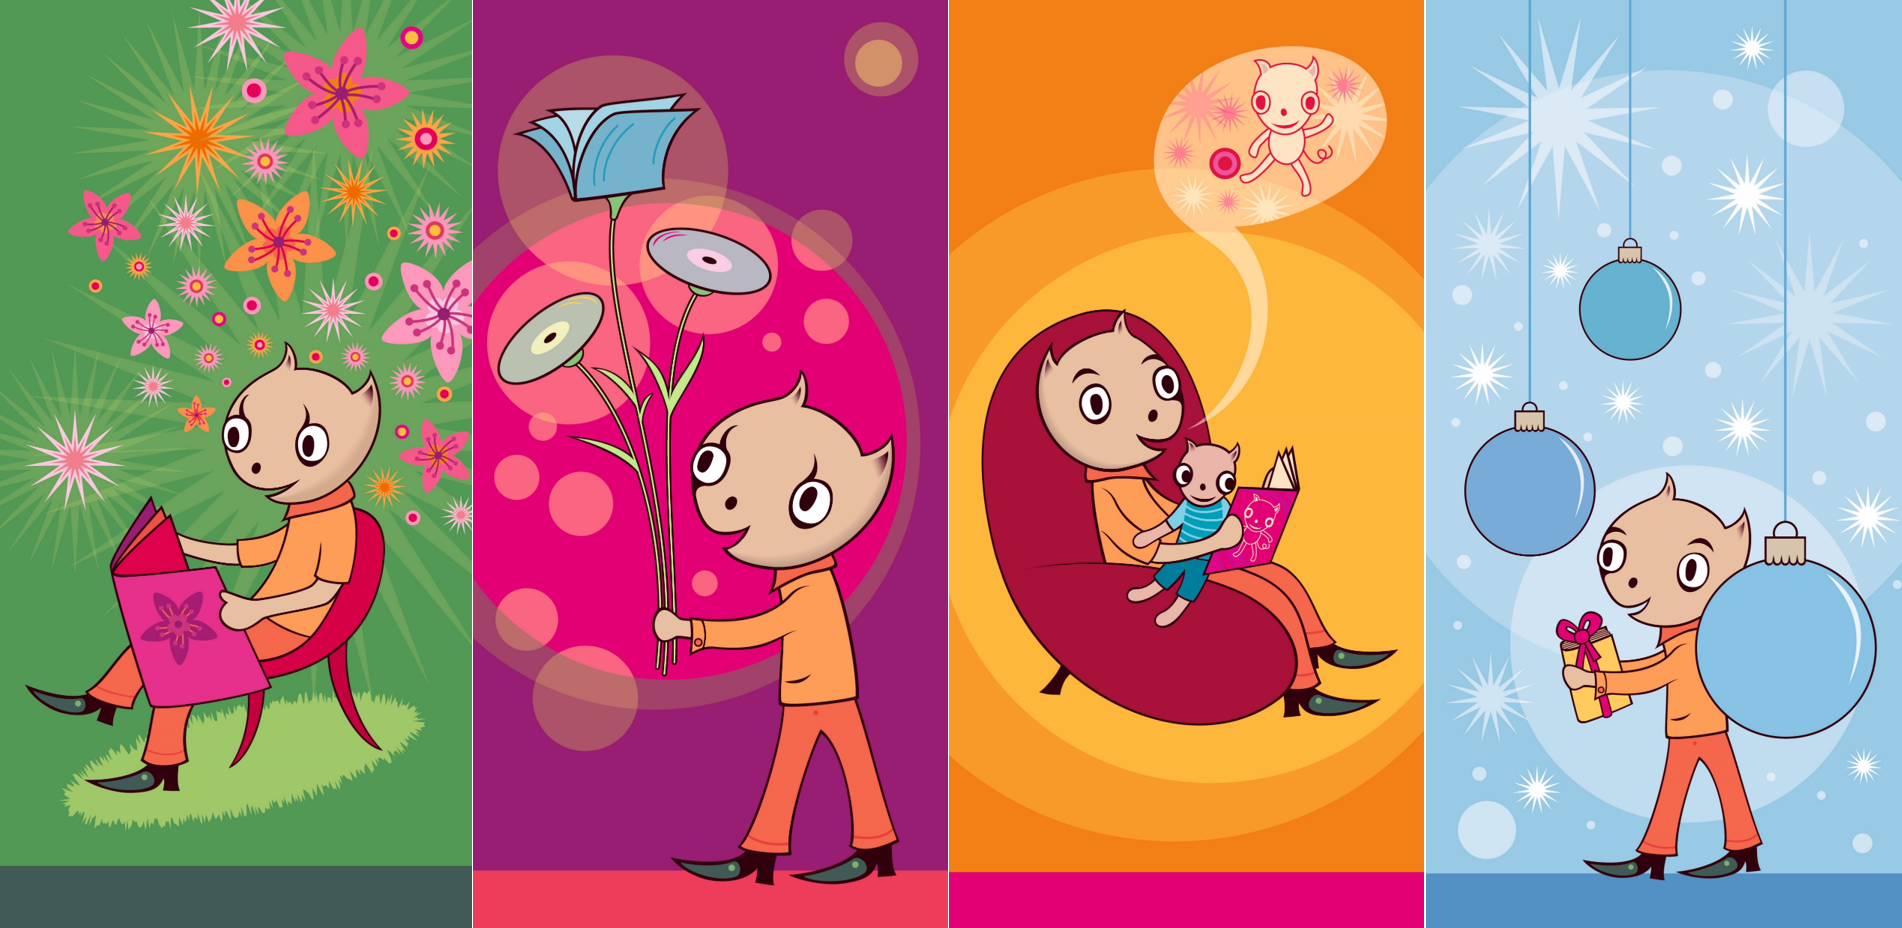
\includegraphics[width=0.9\textwidth]{img/image2.png}
\end{figure}

\emph{LIBREAS: Stachen diese beiden
Projekte für Sie heraus aus Ihrem sonstigen Schaffen oder würden Sie die
eher als typisch für Ihre Projekte ansehen?}

Eigentlich sind es sehr typische Aufträge von mir. Das Thema Bibliothek
fand ich sehr schön und ich hatte bei beiden Aufträgen viele Freiheiten.
Daher waren es besonders schöne Aufträge.

\emph{LIBREAS: Welche Ziele hatten, Ihrer Meinung nach, die Bibliotheken
konkret mit den Projekten? Gab es besondere Herausforderungen zum
Beispiel seitens der Bibliotheksleitungen?}

Die Botschaft der Nationalbibliothek lautet: Übt Sorgfalt mit den
Büchern. Den Kornhausbibliotheken ging es um die Leseförderung und den
Gebrauch der Volksbibliothek durch Kindern und mit den allgemeinen
Geschenkgutscheinen auch durch ein breites Publikum.

Die Zusammenarbeit mit den zuständigen Personen (beim zweiten Auftrag
war es die Bibliotheksleitung) war sehr toll und es gab keine Probleme.

\emph{LIBREAS: Sie haben eine spezifisch anthropomorphe Form der Tiere
gewählt -- die Tiere sind eher Menschen als \enquote{richtige Tiere}.
Das machen auch andere Designer*innen und Künstler*innen. Denken Sie,
nur so sind Tiere und Bibliotheken miteinander zu verbinden? Passen
Tiere als solche sonst nicht zu Bibliotheken?}

In meinen Illustrationen kommen solche Tiermenschen häufig vor. Mir
gefällt diese Form um mich auszudrücken und etwas darzustellen sehr. Ich
finde, bei dieser Bildsprache schaut das Zielpublikum eher hin, als wenn
es ganz menschliche Figuren wären. Und ja, bei \enquote{Tiere als
solchen} würde der Bezug zur Bibliothek vielleicht schon fehlen.

\emph{LIBREAS: Welche konkrete Rolle spielten die von Ihnen gewählten
Tiere bei der Realisierung des Projektes?}

Bei meinen Lesezeichen habe ich mich von der Eule mit den Eigenschaften
der Weisheit, Einsicht, des freundlichen Äusseren für die \enquote{gute}
Figur und für die Leseratte mit der Zuschreibung des Schmutzigen
inspirieren lassen. Ich habe also auch mit bekannten Stereotypen der
Eule und der Ratte gespielt. Und doch soll die Leseratte unbedingt auch
eine sympathische Figur sein, sie ist wissensbegierig, aktiv, kreativ,
liest draussen am Strand, etc. Dies sollte sie aber eben mit den
Bibliotheksbüchern nicht machen, woran eine Leser*in beim Benutzen des
Lesezeichens erinnert wird.

Für mich war es ideal, die Botschaft mit diesen beiden Tieren zu
vermitteln.

\emph{LIBREAS: Welche Erfahrungen nehmen Sie aus den Projekten für die
Zusammenarbeit mit Bibliotheken mit? Würden Sie anderen Designer*innen
raten, auch solche Projekte durchzuführen oder eher nicht?}

Ja, ich würde anderen dazu raten. Es war eine sehr schöne Arbeit, die
ich sofort wieder machen würde. Die Erfahrung war, dass ein breites
Publikum auf meine Arbeit aufmerksam wurde.

%autor
\begin{center}\rule{0.5\linewidth}{0.5pt}\end{center}

\textbf{Judith Zaugg} (*1970) Grafikerin
und Buchherstellerin. Lebt und studierte in Bern. Zahlreiche
Ausstellungen, Stipendien und Preise in der Schweiz, Deutschland und
darüber hinaus. Zahlreiche Kinder- und Bildbücher und weitere eigene
Publikationen sowie Veröffentlichungen in deutschen und schweizerischen
Medien. https://www.judithzaugg.ch, info@judithzaugg.ch

\end{document}
